\documentclass[aspectratio=169]{beamer}
\useoutertheme[progressbar=frametitle]{metropolis}
\useinnertheme{metropolis}
\definecolor{nabgray}{rgb}{0.6,0.59,0.61}
\usecolortheme[named=nabgray]{structure}

\usepackage{tikz}
\usepackage[utf8]{inputenc}
\usepackage[spanish]{babel}
\usepackage{fontspec}
\usepackage{ulem}

\setmonofont{JetBrains Mono}
\setmainfont{Roboto}
\setsansfont{Roboto}


\usepackage{smartdiagram}
\usepackage{qtree}
\usepackage{verbatim}
\usepackage{svg}
\usepackage{graphicx}
\usepackage{color}


\definecolor{lightgray}{rgb}{0.95, 0.95, 0.95}
\definecolor{darkgray}{rgb}{0.4, 0.4, 0.4}
%\definecolor{purple}{rgb}{0.65, 0.12, 0.82}
\definecolor{editorGray}{rgb}{0.95, 0.95, 0.95}
\definecolor{editorOcher}{rgb}{1, 0.5, 0} % #FF7F00 -> rgb(239, 169, 0)
\definecolor{editorGreen}{rgb}{0, 0.5, 0} % #007C00 -> rgb(0, 124, 0)
\definecolor{orange}{rgb}{1,0.45,0.13}
\definecolor{olive}{rgb}{0.17,0.59,0.20}
\definecolor{brown}{rgb}{0.69,0.31,0.31}
\definecolor{purple}{rgb}{0.38,0.18,0.81}
\definecolor{lightblue}{rgb}{0.1,0.57,0.7}
\definecolor{lightred}{rgb}{1,0.4,0.5}
\definecolor{ocherCode}{rgb}{1, 0.5, 0} % #FF7F00 -> rgb(239, 169, 0)
\definecolor{blueCode}{rgb}{0, 0, 0.93} % #0000EE -> rgb(0, 0, 238)
\definecolor{greenCode}{rgb}{0, 0.6, 0} % #009900 -> rgb(0, 153, 0)


\usepackage{upquote}
\usepackage{listings}
\lstdefinelanguage{JavaScript}{
    morekeywords=[1]{break, continue, delete, else, for, function, if, in,
        new, return, this, typeof, var, void, while, with},
    % Literals, primitive types, and reference types.
    morekeywords=[2]{false, null, true, boolean, number, undefined,
        Array, Boolean, Date, Math, Number, String, Object},
    % Built-ins.
    morekeywords=[3]{eval, parseInt, parseFloat, escape, unescape},
    % Basic design
    backgroundcolor=\color{lightgray},
    basicstyle={\small\ttfamily},
    frame=l,
    keywordstyle=\footnotesize\color{blue},
    escapeinside={<@}{@>},
    breaklines=true,
    % Line numbers
    xleftmargin={0.75cm},
    numbers=left,
    stepnumber=1,
    firstnumber=1,
    numberfirstline=true
    % Code design
    identifierstyle=\color{black},
    keywordstyle=\color{ocherCode}\bfseries,
    ndkeywordstyle=\color{greenCode}\bfseries,
    stringstyle=\color{ocherCode}\ttfamily,
    commentstyle=\color{darkgray}\ttfamily,
    tabsize=2,
    showtabs=true,
    showspaces=false,
    showstringspaces=false,
    extendedchars=true,
    breaklines=true
}[keywords, comments, strings]

\colorlet{punct}{red!60!black}
\definecolor{background}{HTML}{EEEEEE}
\definecolor{delim}{RGB}{20,105,176}
\colorlet{numb}{magenta!60!black}

\lstdefinelanguage{json}{
    basicstyle=\normalfont\ttfamily,
    numbers=left,
    numberstyle=\scriptsize,
    stepnumber=1,
    numbersep=8pt,
    showstringspaces=false,
    breaklines=true,
    frame=lines,
    literate=
    *{0}{{{\color{numb}0}}}{1}
    {1}{{{\color{numb}1}}}{1}
    {2}{{{\color{numb}2}}}{1}
    {3}{{{\color{numb}3}}}{1}
    {4}{{{\color{numb}4}}}{1}
    {5}{{{\color{numb}5}}}{1}
    {6}{{{\color{numb}6}}}{1}
    {7}{{{\color{numb}7}}}{1}
    {8}{{{\color{numb}8}}}{1}
    {9}{{{\color{numb}9}}}{1}
    {:}{{{\color{punct}{:}}}}{1}
    {,}{{{\color{punct}{,}}}}{1}
    {\{}{{{\color{delim}{\{}}}}{1}
    {\}}{{{\color{delim}{\}}}}}{1}
    {[}{{{\color{delim}{[}}}}{1}
    {]}{{{\color{delim}{]}}}}{1},
}
\lstset{language=java,
	otherkeywords={var,record},
	% Basic design
	backgroundcolor=\color{lightgray},
	basicstyle={\small\ttfamily},
	frame=l,
	keywordstyle=\footnotesize\color{blue},
	escapeinside={<@}{@>},
	breaklines=true,
	% Line numbers
	xleftmargin={0.75cm},
	numbers=left,
	stepnumber=1,
	firstnumber=1,
	numberfirstline=true
	% Code design
	identifierstyle=\color{black},
	keywordstyle=\color{ocherCode}\bfseries,
	ndkeywordstyle=\color{greenCode}\bfseries,
	stringstyle=\color{ocherCode}\ttfamily,
	commentstyle=\color{darkgray}\ttfamily,
	tabsize=2,
	showtabs=true,
	showspaces=false,
	showstringspaces=false,
	extendedchars=true,
	breaklines=true
}



\usebackgroundtemplate%
{%
    
\includegraphics[width=\paperwidth]{Images/Contenido}%
}


\title{Lenguajes JVM en 2020}
\author{Víctor Orozco}
\institute{Academik}
\date{\today}
\begin{document}

{
    \usebackgroundtemplate{
\includegraphics[width=\paperwidth]{Images/Contenido}}
    \setbeamercolor{frametitle}{fg=red}
    \usebeamercolor[fg]{normal text}
    \frame{\titlepage}
}


\begin{frame}
    \huge ¿Para que aprender otros lenguajes de programación si ya existe JavaScript?
\end{frame}


\begin{frame}
    \begin{figure}
        \centering
        
\includegraphics[width=0.5\linewidth]{Images/javavsjs}
    \end{figure}
\end{frame}

\section{Evolución de los lenguajes de programación}

\begin{frame}{Clasificación de los lenguajes de programación}
	\begin{itemize}
		\item Generaciones
		\item Paradigmas
		\item Aplicaciones y usos
	\end{itemize}
\end{frame}

\begin{frame}{Generaciones}
    \smartdiagramset{font = \tiny, priority arrow width=1cm,priority arrow height advance=1.25cm}
     \smartdiagramanimated[priority descriptive diagram]{1GL (Binario), 2GL (ASM), 3GL(Java\, Python\, Basic)}
\end{frame}

\begin{frame}{Generaciones}
    \smartdiagramset{font = \tiny, priority arrow width=1cm,priority arrow height advance=1.25cm}
     \smartdiagram[priority descriptive diagram]{4GL(SQL\, R\, Bash), 5GL (Mercury)}
\end{frame}


\begin{frame}{Paradigmas (Simplificación)}

\Tree[.Paradigmas [.Imperativo [.Estructurado \textit{Pascal} ]
               [.OOP  \textit{Java} ]]
          [.Declarativo [.Funcional \textit{Clojure} ]
                [.Logico \textit{Prolog} ]]]
\end{frame}

\begin{frame}{Aplicaciones y usos}
	\begin{itemize}
	\item 60s-80s Mainframes - RPG (AS/400), COBOL (z/OS, VME)
	\item 80s-2000s Un lenguaje para dominar a todos - Java, Basic, C\#, Pascal
	\item 2010 Especialización de los lenguajes - Kotlin (móvil), Data Science (Python), Web (JavaScript), Infraestructura (Go), Backend (Java)
	\end{itemize}
\end{frame}

\section{Evolución de las plataformas de programación}

\begin{frame}{Lenguaje}
    ¡Yo programo en Java!
\end{frame}

\begin{frame}{Lenguaje}
    ¡Yo programo en el lenguaje Java!
\end{frame}


\begin{frame}{Lenguaje}
    ¡Yo programo en (una de) las plataformas Java!
\end{frame}


\begin{frame}{Lenguaje != Plataforma}
    \sout{Lenguaje}, Plataforma
	\begin{itemize}
	\item Compilador
    \item Entorno de ejecución
    \item APIS y bibliotecas
    \item Frameworks
    \item Editor o IDE
	\end{itemize}
\end{frame}

\begin{frame}{Lenguaje != Plataforma}
    Turbo Pascal

    \begin{columns}[T] % contents are top vertically aligned
	     \begin{column}[T]{0.5\textwidth} % each column can also be its own environment
            \begin{itemize}
                \item Compilador: Borland Pascal
                \item Bibliotecas y APIs: Borland -e.g. conio.h-
                \item Editor: Borland
            \end{itemize}
	     \end{column}
	     \begin{column}[T]{7cm} % alternative top-align that's better for graphics
   			\begin{figure}
   			\centering
   			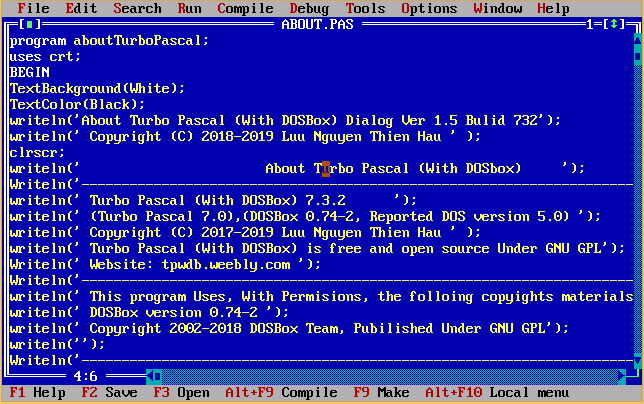
\includegraphics[width=\linewidth]{Images/pascal}
   			\end{figure}

	     \end{column}
     \end{columns}
\end{frame}

\begin{frame}{Lenguaje != Plataforma}
    Visual Basic


    \begin{columns}[T] % contents are top vertically aligned
	     \begin{column}[T]{0.5\textwidth} % each column can also be its own environment
            \begin{itemize}
            	\item Compilador: Microsoft Basic
                \item Bibliotecas y APIs: Microsoft -e.g. Win32, COM, .net-
                \item Editor: Microsoft Visual Studio
            \end{itemize}
	     \end{column}
	     \begin{column}[T]{7cm} % alternative top-align that's better for graphics
      			\begin{figure}
      			\centering
      			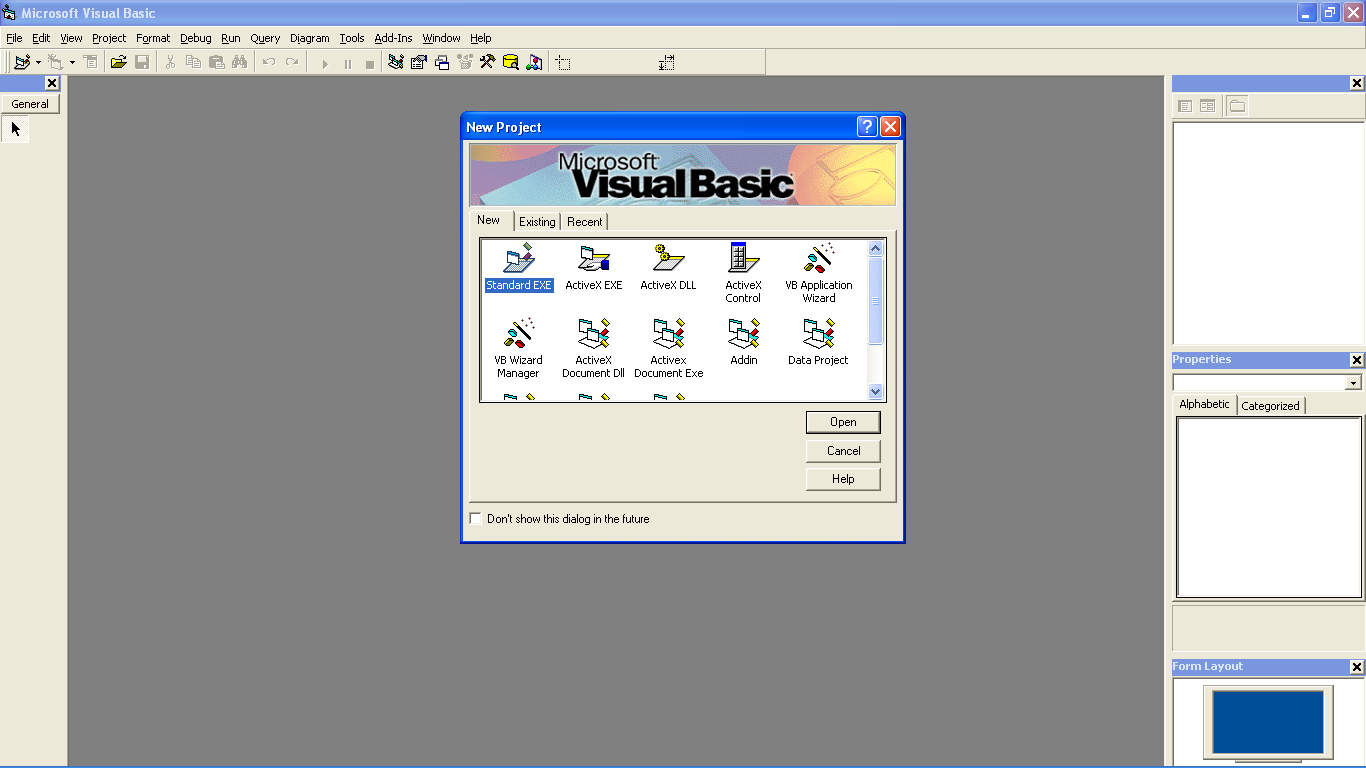
\includegraphics[width=\linewidth]{Images/basic}
      			\end{figure}

	     \end{column}
     \end{columns}

\end{frame}

\begin{frame}{Lenguaje != Plataforma}
    C++
	\begin{itemize}
	\item Compilador: GCC(GNU), Clang(LLVM/Apple), MSVC (Microsoft)
    \item Bibliotecas y APIs: C++ 11 (estandares), musl (Linux), glibc (GNU)
    \item Frameworks: QT
    \item Editor: XCode(Apple), Visual Studio (Microsoft), CLion (JetBrains), QT Creator (Digia)
	\end{itemize}
\end{frame}

\begin{frame}{Lenguaje != Plataforma}
    Java
	\begin{itemize}
	\item Compilador: javac (OpenJDK), incremental(Eclipse JDT)
    \item Entorno ejecución: JVM -e.g. Oracle HotSpot, Amazon Correto, RedHat OpenJDK, IBM J9-, Nativo (GraalVM)
    \item Bibliotecas y APIs: OpenJDK (estandares) (Oracle, Google, RedHat), Maven Central
    \item Frameworks: Spring (VMWare), Jakarta EE (Oracle, RedHat)
    \item Editor: NetBeans (Apache), Eclipse (Eclipse), IntelliJ IDEA (JetBrains), VSCode (Microsoft)
	\end{itemize}
\end{frame}

\section{Lenguajes JVM}
\begin{frame}{JVM}
	JVM

	\begin{columns}[T] % contents are top vertically aligned
		\begin{column}[T]{0.5\textwidth} % each column can also be its own environment
			\begin{itemize}
				\item \textbf{25 años de desarrollo}
				\item Nueva versión cada 6 meses
				\item Software libre GPLv2+Classpath Exception
				\item Probablemente la maquina virtual más rápida
			\end{itemize}
		\end{column}
		\begin{column}[T]{7cm} % alternative top-align that's better for graphics
			\begin{figure}
				\centering
				
\includegraphics[width=\linewidth]{Images/openjdk}
			\end{figure}

		\end{column}
	\end{columns}
\end{frame}
\begin{frame}{}
	\begin{figure}
		\centering
		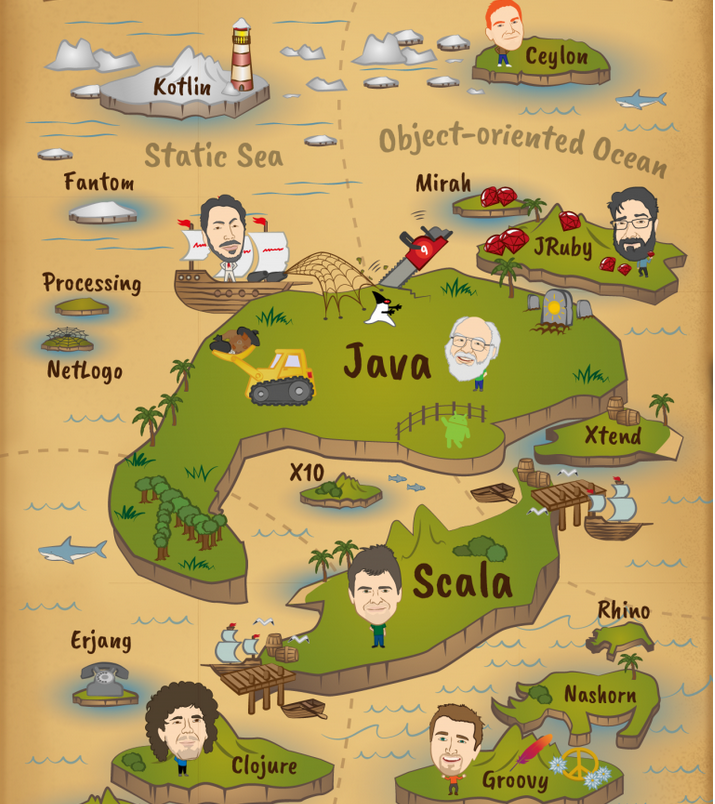
\includegraphics[width=0.5\linewidth]{Images/pirates}
	\end{figure}

\end{frame}

\begin{frame}{JVM}
	Snyk - JVM Ecosystem report 2020

	\begin{figure}
		\centering
		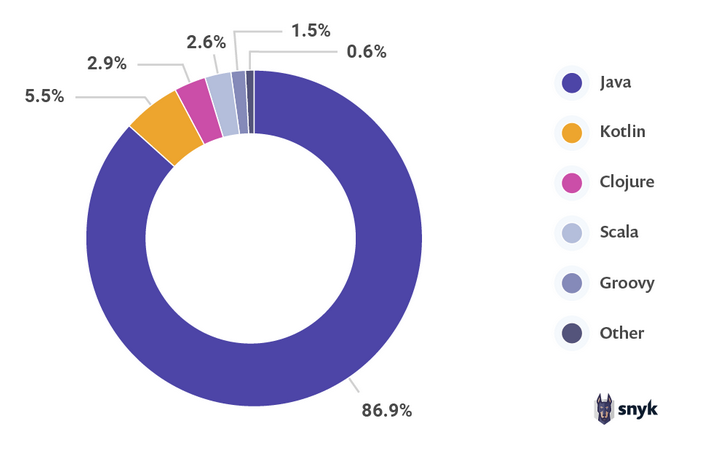
\includegraphics[width=0.7\linewidth]{Images/jvmlangs}
	\end{figure}

\end{frame}

\begin{frame}{Java}
	\begin{columns}[T] % contents are top vertically aligned
		\begin{column}[T]{0.5\textwidth} % each column can also be its own environment
			\begin{itemize}
				\item Creado en: 1996
				\item Paradigma: Orientado a objetos, funcional, reflectivo, concurrente
				\item Tipado: Fuerte, estático
				\item Plataformas: JVM, JavaScript (GWT), Nativo (GraalVM Native)
                \item Popular en: Data Engineering, Backend, Móvil (Android)
				\item Usuarios importantes: NASDAQ, Spotify, SAT
			\end{itemize}
		\end{column}
		\begin{column}[T]{7cm} % alternative top-align that's better for graphics
			\begin{figure}
				\centering
				
\includegraphics[width=\linewidth]{Images/java}
			\end{figure}

		\end{column}
	\end{columns}
\end{frame}

\begin{frame}[fragile]{Java}
\begin{lstlisting}
public class Hello {

    public static void main(String args[]) {
        System.out.println("Hola mundo");
    }
}
\end{lstlisting}
\end{frame}


\begin{frame}{Kotlin}
	\begin{columns}[T] % contents are top vertically aligned
		\begin{column}[T]{0.5\textwidth} % each column can also be its own environment
			\begin{itemize}
				\item Creado en: 2011
				\item Paradigma: Orientado a objetos, funcional, reflectivo
				\item Tipado: Fuerte, estático, inferencia
				\item Plataformas: JVM, JavaScript, Nativo(LLVM), Nativo (GraalVM Native)
				\item Popular en: Móvil (Android)
				\item Usuarios importantes: JetBrains, Healthcare.com
			\end{itemize}
		\end{column}
		\begin{column}[T]{7cm} % alternative top-align that's better for graphics
			\begin{figure}
				\centering
				
\includegraphics[width=0.5\linewidth]{Images/kotlin}
			\end{figure}

		\end{column}
	\end{columns}
\end{frame}

\begin{frame}[fragile]{Kotlin}
\begin{lstlisting}
fun main() {
    val scope = "World"
    println("Hello, $scope!")
}
\end{lstlisting}
\end{frame}



\begin{frame}{Clojure}
	\begin{columns}[T] % contents are top vertically aligned
		\begin{column}[T]{0.5\textwidth} % each column can also be its own environment
			\begin{itemize}
				\item Creado en: 2007
				\item Paradigma: Funcional, lógico
				\item Tipado: Fuerte, dinámico
				\item Plataformas: JVM, JavaScript, CLR (.net)
				\item Popular en: Backend
				\item Usuarios importantes: Nubank
			\end{itemize}
		\end{column}
		\begin{column}[T]{7cm} % alternative top-align that's better for graphics
			\begin{figure}
				\centering
				
\includegraphics[width=0.5\linewidth]{Images/clojure}
			\end{figure}

		\end{column}
	\end{columns}
\end{frame}

\begin{frame}[fragile]{Clojure}
\begin{lstlisting}
(defn -main ; name
  [& args] ; (variable) parameters
  (println "Hello, World!")) ; body
\end{lstlisting}
\end{frame}


\begin{frame}{Scala}
	\begin{columns}[T] % contents are top vertically aligned
		\begin{column}[T]{0.5\textwidth} % each column can also be its own environment
			\begin{itemize}
				\item Creado en: 2004
				\item Paradigma: Orientado a objetos, funcional, reflectivo
				\item Tipado: Fuerte, estático, inferencia
				\item Plataformas: JVM, JavaScript, Nativo (GraalVM Native)
				\item Popular en: Data Engineering (Spark, Hadoop), Backend
				\item Usuarios importantes: Spotify, Reuters
			\end{itemize}
		\end{column}
		\begin{column}[T]{7cm} % alternative top-align that's better for graphics
			\begin{figure}
				\centering
				
\includegraphics[width=0.5\linewidth]{Images/scala}
			\end{figure}

		\end{column}
	\end{columns}
\end{frame}

\begin{frame}[fragile]{Scala}
\begin{lstlisting}
object HelloWorld extends App {
   println("Hello, World!")
}
\end{lstlisting}
\end{frame}


\begin{frame}{Groovy}
	\begin{columns}[T] % contents are top vertically aligned
		\begin{column}[T]{0.5\textwidth} % each column can also be its own environment
			\begin{itemize}
				\item Creado en: 2003
				\item Paradigma: Orientado a objetos, funcional, reflectivo, scripting
				\item Tipado: Fuerte, dinámico, inferencia
				\item Plataformas: JVM, JavaScript(Grooscript)
				\item Popular en: Infra, Backend, Android
				\item Usuarios importantes: Google, Jenkins, LinkedIn, Gradle
			\end{itemize}
		\end{column}
		\begin{column}[T]{7cm} % alternative top-align that's better for graphics
			\begin{figure}
				\centering
				
\includegraphics[width=0.5\linewidth]{Images/groovy}
			\end{figure}

		\end{column}
	\end{columns}
\end{frame}

\begin{frame}[fragile]{Groovy}
\begin{lstlisting}
print "Hello World!\n"
\end{lstlisting}
\end{frame}



\section{Plataforma}

\begin{frame}{Plataformas}
    Móvil
	\begin{itemize}
	\item Android nativo: Java, Kotlin, C++
    \item iOS nativo: Swift, Objective-C
    \item Multiplataforma web: JavaScript (Ionic, Cordova)
    \item Multiplataforma nativa: JavaScript (React), Java (Gluon/JavaFX), C\# (Xamarin), Dart(Flutter)
	\end{itemize}
\end{frame}

\begin{frame}{Plataformas}
    Escritorio
	\begin{itemize}
	\item Nativo APIs: Winforms (C\#, Basic), Cocoa (Swift, Objective-C), GTK (Python, Vala, C++)
    \item Multiplataforma: Electron (JavaScript, TypeScript), Swing/JavaFX (Java, Kotlin, Scala), GTK (Python, Vala, C++), QT (C++, Python)
	\end{itemize}
\end{frame}



\begin{frame}{Plataformas}
    Backend/procesamiento de datos
	\begin{itemize}
	\item Big Data: Spark, Hadoop, Kafka, Storm (Scala, Java)
    \item Data Science: Tensorflow, PyTorch, Keras (Python)
    \item Tradicional: Java (Spring/Java EE), PHP, .net
    \item Microservicios: Java (Spring Boot/MicroProfile), JavaScript (Node, Deno), .net (Core)

	\end{itemize}
\end{frame}

\begin{frame}{Plataformas}

	\begin{alertblock}{Desarrollar software en 2020}
    Cada día que pasa es más difícil la existencia de un lenguaje de propósito general y la tendencia es lenguajes generales para propósitos específicos.
	\end{alertblock}
\end{frame}

\begin{frame}{Plataformas}

	\begin{alertblock}{Desarrollar software en 2020}
    El presente del desarrollo de software es eminentemente políglota y flexible. Ya no existe y probablemente ya no existirá un entorno para dominarlos a todos.
	\end{alertblock}
\end{frame}

\section{Tendencias políglotas}

\begin{frame}{.net framework (2002)}

	\begin{figure}
    			\centering
    			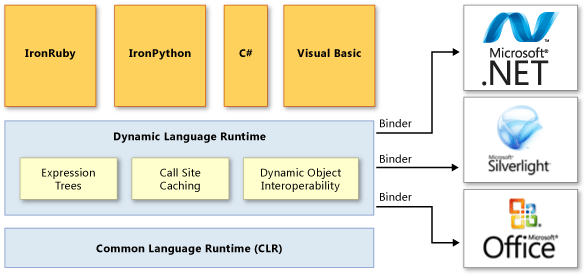
\includegraphics[width=\linewidth]{Images/netpoly}
    			\end{figure}

\end{frame}

\begin{frame}{Parrot VM (2016)}

	\begin{figure}
    			\centering
    			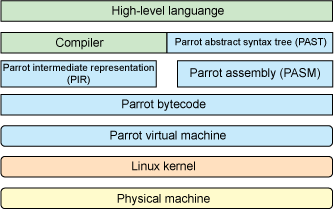
\includegraphics[width=0.6\linewidth]{Images/parrot}
    \end{figure}

\end{frame}

\begin{frame}{GraalVM (2019)}

	\begin{figure}
		\centering
		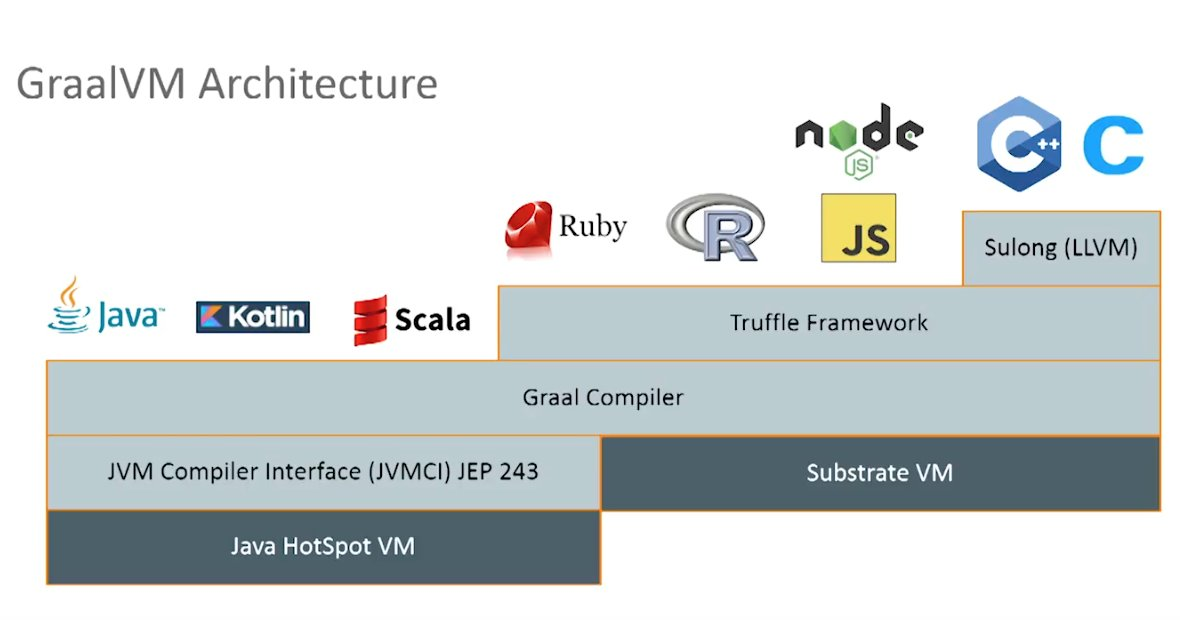
\includegraphics[width=\linewidth]{Images/graalvm}
	\end{figure}

\end{frame}

\begin{frame}{Microservicios (Netflix)}

	\begin{figure}
		\centering
		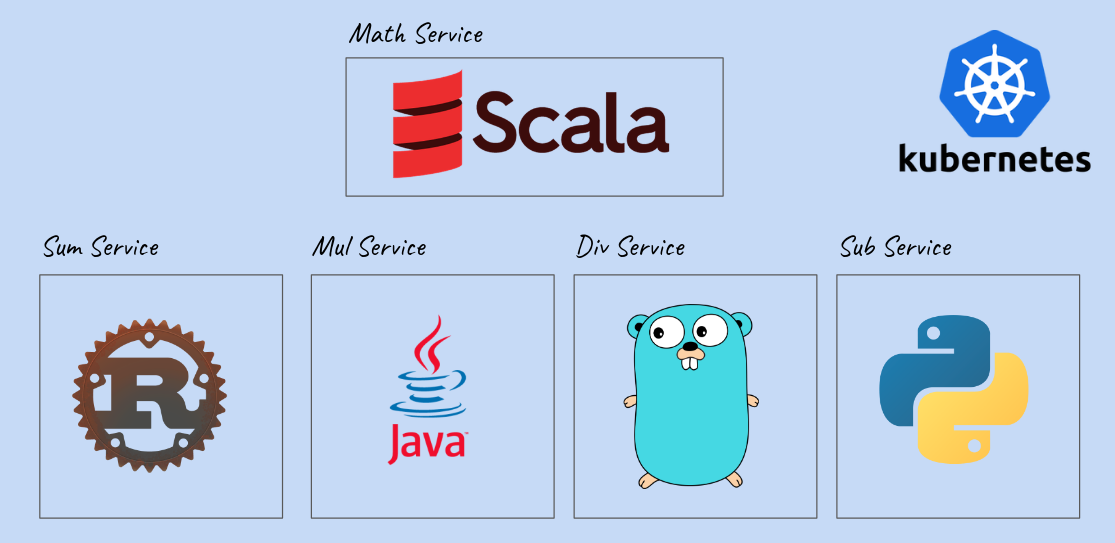
\includegraphics[width=\linewidth]{Images/microservices}
	\end{figure}

\end{frame}




\section{Principios de sobrevivencia en un múndo políglota}

\begin{frame}{Principios de sobrevivencia}

	\begin{exampleblock}{Principio \#0: Utilidad real de los lenguajes de programación}
    Al final del día lo que la computadora entiende es lenguaje máquina. Los lenguajes de programación sirven para comunicarnos entre programadores.
	\end{exampleblock}
\end{frame}


\begin{frame}{Principios de sobrevivencia}

	\begin{exampleblock}{Principio \#1: Especialización de los lenguajes}
    Contrario a lo que se piensa o se enseña en la universidad, los lenguajes de programación ya no son \textit{iguales}.
	\end{exampleblock}
\end{frame}


\begin{frame}{Principios de sobrevivencia}

	\begin{exampleblock}{Principio \#2: Paradigmas sobre lenguaje}
    En el largo plazo es más conveniente entender un paradigma de programación que un lenguaje en particular.
	\end{exampleblock}
\end{frame}

\begin{frame}{Principios de sobrevivencia}

	\begin{exampleblock}{Principio \#3: Diferentes paradigmas = Mejores habilidades}
    Un buen mínimo para prepararse para el futuro y el presente:
    \begin{itemize}
    	\item Tipado fuerte: Java (C++, C\#, Kotlin, Scala, Dart, Swift, Go, Rust, TypeScript)
        \item Tipado dinámico: JavaScript, Python (Ruby, Julia, Lisp, Clojure)
        \item Scripting: Bash (simple), Powershell (POO)
        \item Consulta de datos: SQL
   	\end{itemize}

	\end{exampleblock}
\end{frame}

\begin{frame}{Principios de sobrevivencia - Tiobe}
	\begin{figure}
		\centering
		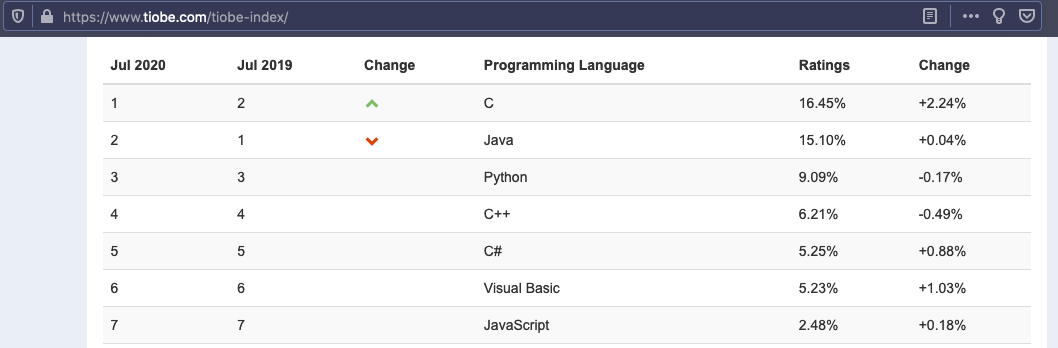
\includegraphics[width=0.9\linewidth]{Images/tiobe}
	\end{figure}
\end{frame}

\begin{frame}{Principios de sobrevivencia - IEEE}
    \begin{figure}
        \centering
        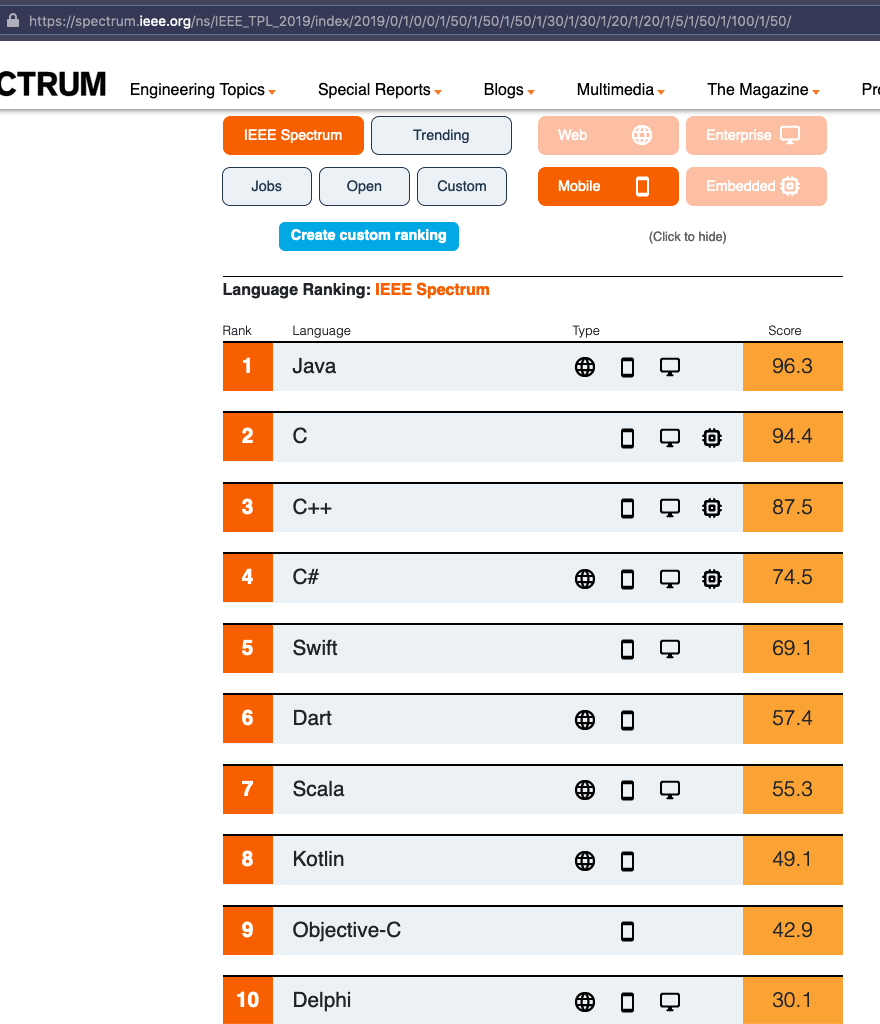
\includegraphics[width=0.5\linewidth]{Images/ieeemobile}
    \end{figure}
\end{frame}

\begin{frame}{Principios de sobrevivencia - IEEE}
    \begin{figure}
        \centering
        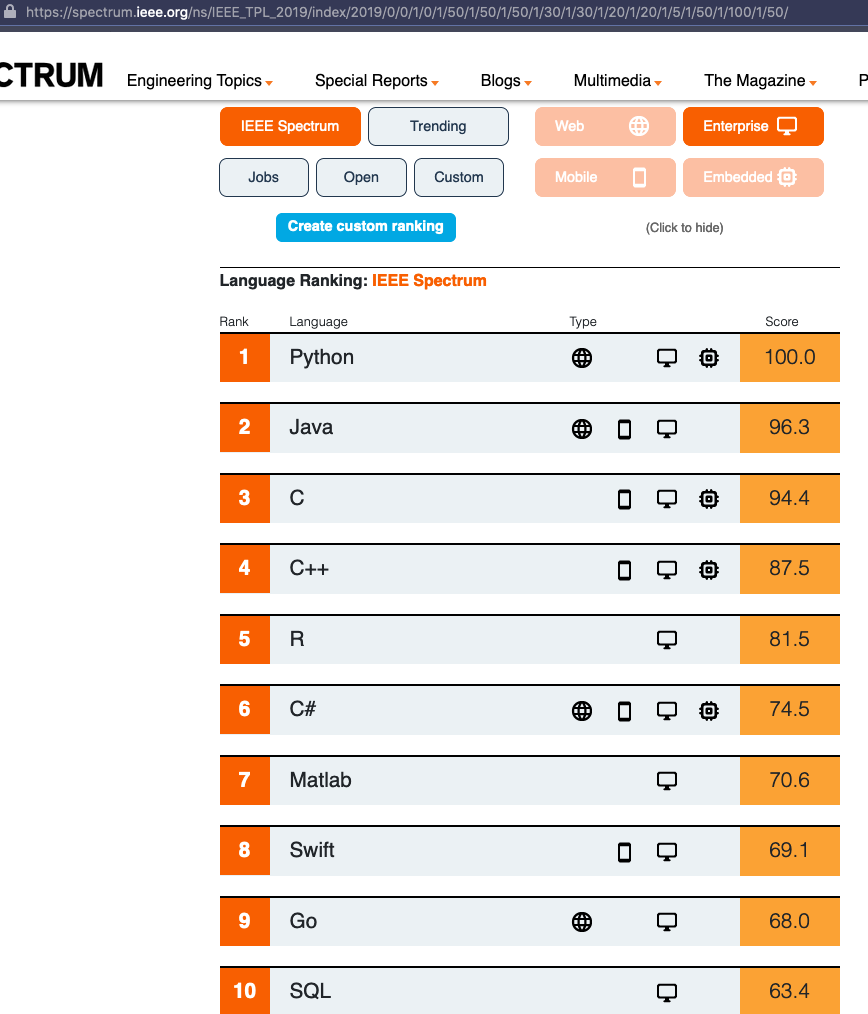
\includegraphics[width=0.5\linewidth]{Images/ieeeenterpise}
    \end{figure}
\end{frame}

\begin{frame}{Principios de sobrevivencia - Forbes}
    \begin{figure}
        \centering
        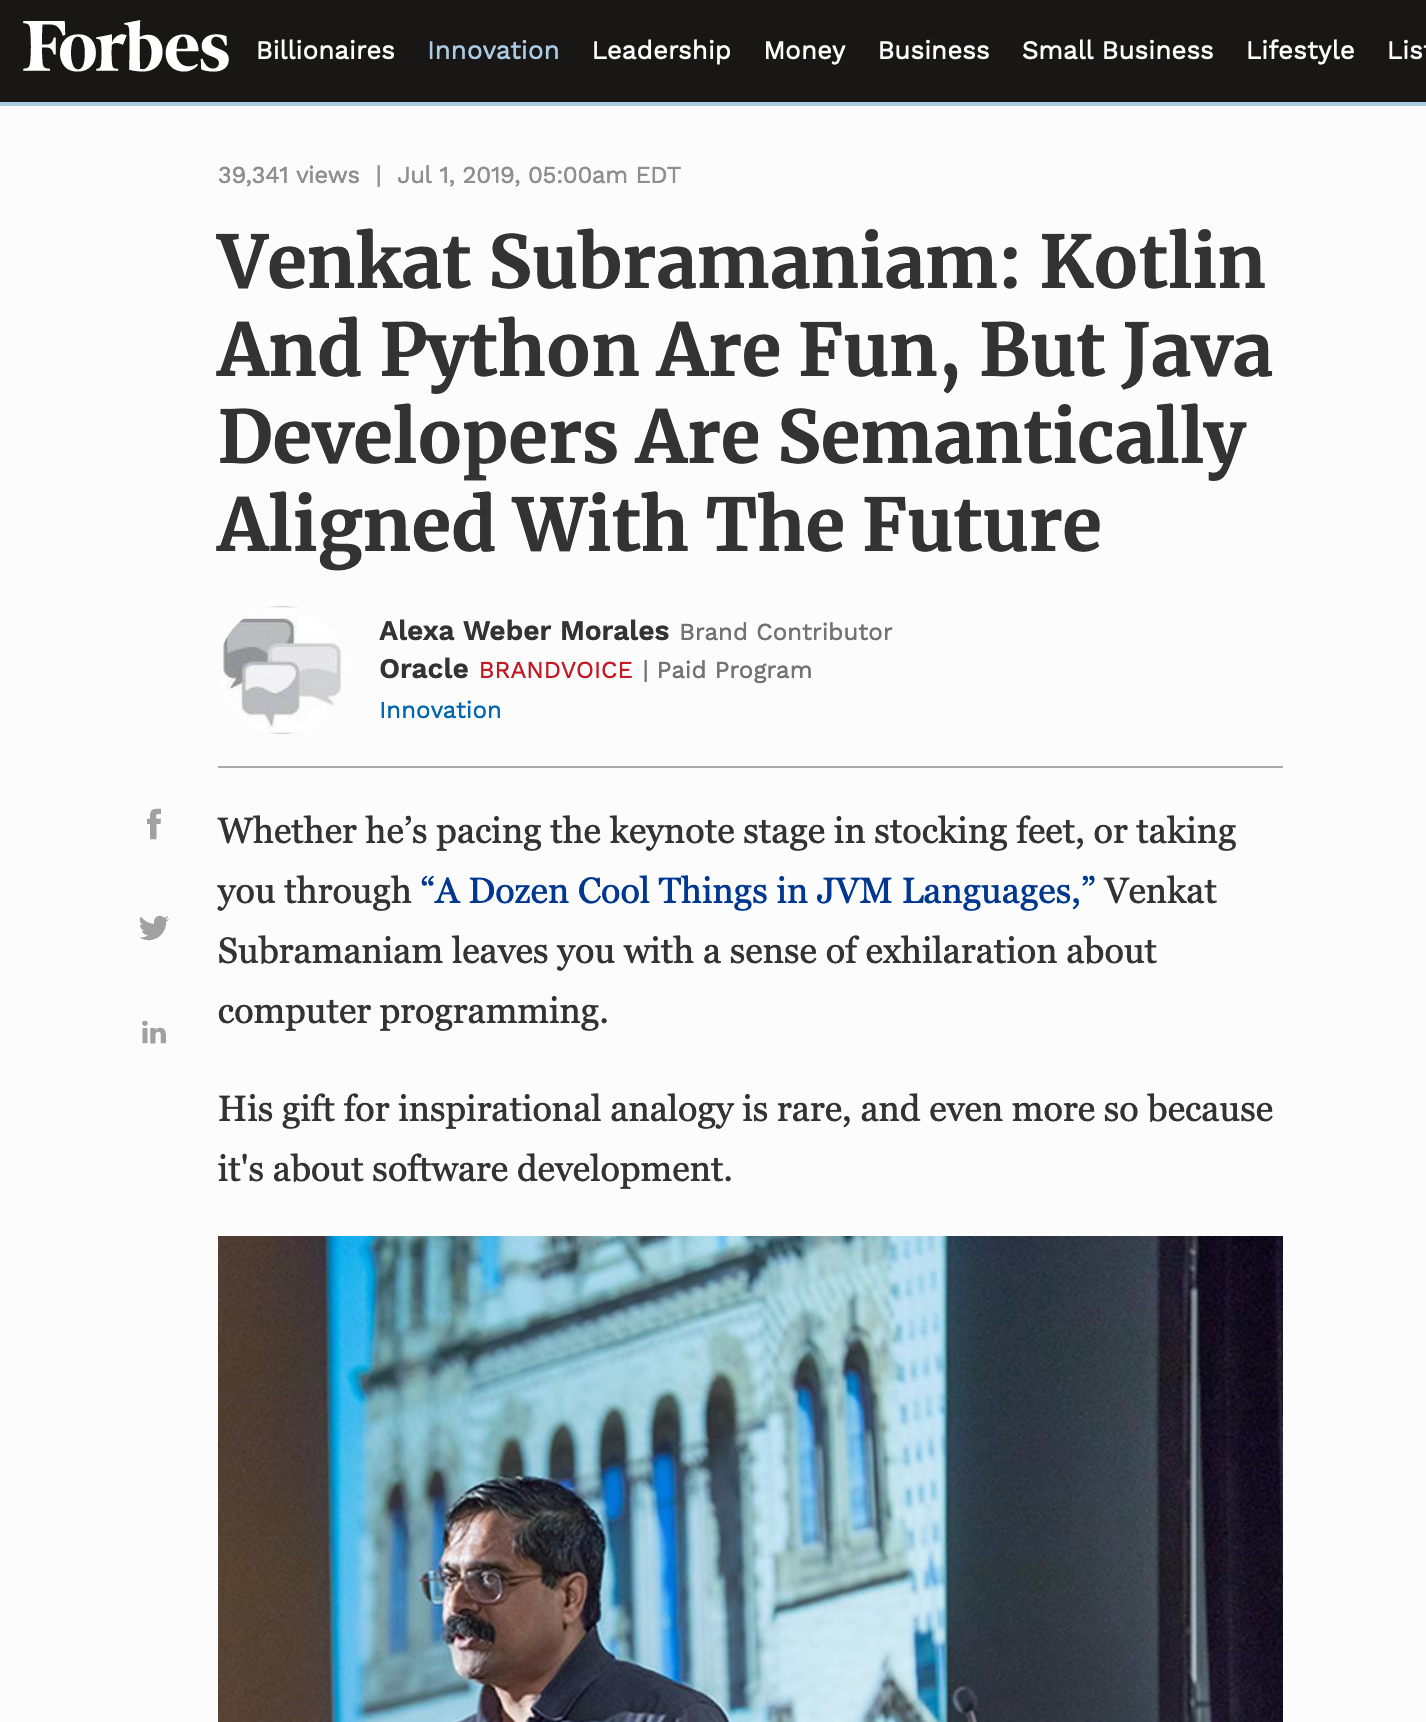
\includegraphics[width=0.5\linewidth]{Images/venkat}
    \end{figure}
\end{frame}

\begin{frame}{Víctor Orozco}
    \begin{columns}[T] % contents are top vertically aligned

        \begin{column}[T]{4cm} % alternative top-align that's better for graphics
            \begin{figure}
                \centering
                
\includegraphics[width=\linewidth]{Images/logos}
            \end{figure}
        \end{column}
        \begin{column}[T]{6cm} % each column can also be its own environment
            \begin{itemize}
                \item vorozco@nabenik.com
                \item \href{https://twitter.com/tuxtor}{@tuxtor}
                \item \href{http://vorozco.com}{http://vorozco.com}
                \item \href{http://tuxtor.shekalug.org}{http://tuxtor.shekalug.org}
            \end{itemize}
            \begin{center}
                
\includegraphics[width=0.1\linewidth]{Images/cclogo}
                \\
                This work is licensed under Creative Commons Attribution-NonCommercial-ShareAlike 3.0 Guatemala (CC BY-NC-SA 3.0 GT).
            \end{center}
        \end{column}
    \end{columns}
\end{frame}



\end{document}

